\chapter{Introduction to \texttt{python}}\label{introduction-to-python---lesson-1}

$\tt{Python}$ is one of the most widely used programming languages in the world, and it has been around for almost 30 years now~\cite{survey2019}.

First and foremost reason why $\tt{python}$ is much popular because it is highly productive as compared to other programming languages like $\tt{C++}$ and $\tt{java}$. It is a much more concise and expressive language and requires less time, effort, and lines of code to perform the same operations.

This makes $\tt{python}$ a very easy-to-learn programming language even for beginners and newbies. It is also very famous for its simple programming syntax, code readability and English-like commands that make coding in \texttt{python} lot easier and efficient.
With $\tt{python}$, the code looks very close to how humans think. For this purpose, it must abstract the details of the computer from you. Hence, it is slower than other “lower-level language” like $\tt{C}$.

There were times when computer run-time used to be the main issue and the most expensive resource. But now, things have changed. Computer, servers and other hardware have become much much cheaper than ever and speed has become a less important factor. Today, development time matters more in most cases rather than execution speed. Reducing the time needed for each project saves companies tons of money.

As far as the execution speed or performance of the program is concerned, we can easily manage it by horizontal scaling, meaning that more servers can be used to reach that level of speed or performance.

In short, $\tt{python}$ is widely used even when it is somehow slower than other languages because:
\begin{itemize}
	\tightlist
  \item is more productive;
  \item companies can optimize their most expensive resource: employees;
  \item rich set of libraries and frameworks;
  \item large community.
\end{itemize}

\begin{figure}[!ht]
	\centering
	\subfloat[Most used programming languages.\label{subfig-1:used}]{%
		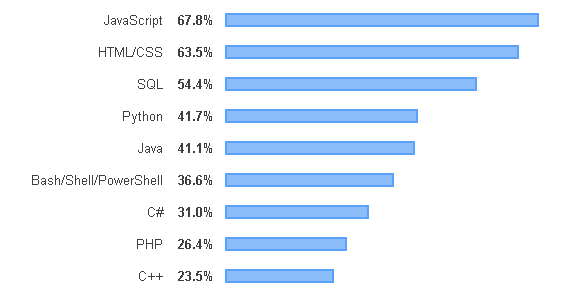
\includegraphics[width=0.7\textwidth]{figures/most_used}
	}\\
	\subfloat[Most loved programming languages.\label{subfig-2:loved}]{%
		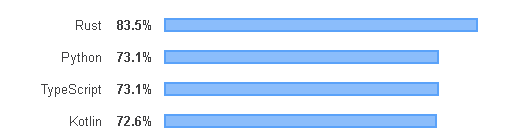
\includegraphics[width=0.7\textwidth]{figures/most_loved}
	}\\
	\subfloat[Most dreaded programming languages.\label{subfig-3:dreaded}]{%
	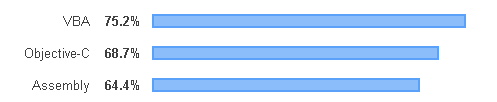
\includegraphics[width=0.7\textwidth]{figures/most_dreaded}
	}
	\caption{Results from 2019 Stack Overflow survey.}
	\label{fig:dummy}
\end{figure}

\section{What is $\tt{python}$ ?}\label{what-is-python}

$\tt{python}$ is a so called \emph{interpreted language}: it takes some code (a sequence of instructions), reads and executes it. This is different from other programming languages like \texttt{C} or \texttt{C++} which \emph{compile} code into a language that computers can understand directly (\emph{machine language}) (see Fig.~\ref{fig:compiled_vs_interpreted}).

\begin{figure}[h]
\centering
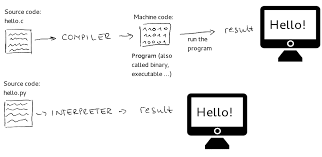
\includegraphics[width=0.7\linewidth]{figures/index.png}
\caption{Interpreted vs compiled language.}
\label{fig:compiled_vs_interpreted}
\end{figure}

As a result, \(\tt{python}\) is essentially an \emph{interactive} programming language, which means you can program and see the results almost at the same time. This is very nice for a faster development since "compilation" time can be quite long (just to give an idea the compilation of our \texttt{C++} financial code takes more than one hour).
However there are drawbacks in term of performance, the \emph{translation} to machine language has to be done in real-time resulting in slower execution times (see Fig.~\ref{fig:compilation}).

\begin{figure}[h]
\centering
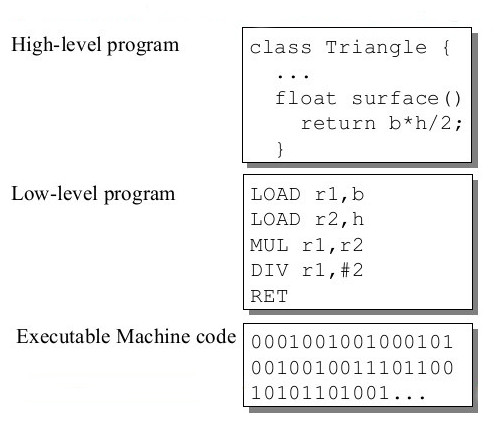
\includegraphics[width=0.5\linewidth]{figures/machine_language.jpeg}
\caption{Human readable vs machine code}
\label{fig:compilation}
\end{figure}

In the next Chapters we'll take a quick tour of $\tt{python}$ and see the main features and characteristics of this programming language. Later on we will see how it can be useful to solve real-world financial problems.

First of all since $\tt{python}$, as basically all programs, comes in different version and flavours we need to specify the particular one we are going to use~\cite{python_versions}.
The latest version (at the time I'm writing this pages) is \(\tt{3.8.5}\), however it is still not difficult to see older versions floating around (e.g. \(\tt{2.7}\)).
This is because there are some big differences between \(\tt{python 2.X}\) and \(\tt{python 3.X}\) which prevent a sizable portion of \(\tt{python 2}\) users to stick with it (consider that moving to \(\tt{python 3}\) would require a large amount of work to adapt big projects).
In conclusion we will concentrate on \textbf{\(\tt{python~3.7}\)}.

\section{$\tt{python}$ Basics}\label{python-basics}

Every language has \emph{keywords}, these are reserved words that have special meaning and tell the computer what to do. The first one we encounter is \(\tt{print}\): it prints to screen whatever is specified between the parenthesis.

\begin{codebox}
\begin{Verbatim}[commandchars=\\\{\}]
\PY{n+nb}{print} \PY{p}{(}\PY{l+s+s2}{\PYZdq{}}\PY{l+s+s2}{Hello world !}\PY{l+s+s2}{\PYZdq{}}\PY{p}{)} 

Hello world !
\end{Verbatim}
\end{codebox}

\begin{codebox}
\begin{Verbatim}[commandchars=\\\{\}]
\PY{n+nb}{print} \PY{p}{(}\PY{l+s+s2}{\PYZdq{}}\PY{l+s+s2}{Welcome}\PY{l+s+s2}{\PYZdq{}}\PY{p}{)}
\PY{n+nb}{print} \PY{p}{(}\PY{l+s+s2}{\PYZdq{}}\PY{l+s+s2}{to}\PY{l+s+s2}{\PYZdq{}}\PY{p}{)}
\PY{n+nb}{print} \PY{p}{(}\PY{l+s+s2}{\PYZdq{}}\PY{l+s+s2}{everybody}\PY{l+s+s2}{\PYZdq{}}\PY{p}{)}

Welcome
to
everybody
\end{Verbatim}
\end{codebox}

Good programming practice recommends to document the code you write (you will soon see that it is surprisingly easy to forget what you wanted to do in your code). In \(\tt{python}\) you can add comments to code starting a line with a hash character (\#).

\begin{codebox}
\begin{Verbatim}[commandchars=\\\{\}]
\PY{n+nb}{print} \PY{p}{(}\PY{l+s+s2}{\PYZdq{}}\PY{l+s+s2}{Ciao}\PY{l+s+s2}{\PYZdq{}}\PY{p}{)} \PY{c+c1}{\PYZsh{} this is a comment}

Ciao
\end{Verbatim}
\end{codebox}

\subsection{Variables}\label{variables}

A variable is a computer memory location paired with a symbolic name, which contains some quantity of information referred to as a \emph{value} (e.g. a number, a string\ldots). Variables and hence data they contain, can be used, referenced and manipulated throughout a program.
A value is assigned to a variable with the equal operator (=) and printing a variable shows its content. 

\begin{figure}[h]
\centering
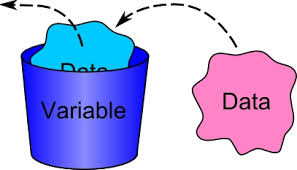
\includegraphics[width=0.35\linewidth]{figures/var1.jpeg}\\
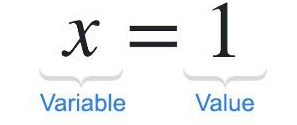
\includegraphics[width=0.35\linewidth]{figures/var2.jpeg}
\caption{Graphical representation of a variable.}
\end{figure}

\begin{codebox}
\begin{Verbatim}[commandchars=\\\{\}]
\PY{n}{x} \PY{o}{=} \PY{l+m+mi}{9}
\PY{n+nb}{print} \PY{p}{(}\PY{n}{x}\PY{p}{)}

9
\end{Verbatim}
\end{codebox}

\begin{codebox}
\begin{Verbatim}[commandchars=\\\{\}]
\PY{n}{myphone} \PY{o}{=} \PY{l+s+s2}{\PYZdq{}}\PY{l+s+s2}{Huawei P10Lite}\PY{l+s+s2}{\PYZdq{}}
\PY{n+nb}{print} \PY{p}{(}\PY{n}{myphone}\PY{p}{)}

Huawei P10Lite
\end{Verbatim}
\end{codebox}

Another very useful keyword is \(\tt{type}\): it tells which kind of object is stored in a variable.

\begin{codebox}
\begin{Verbatim}[commandchars=\\\{\}]
\PY{n+nb}{print} \PY{p}{(}\PY{n+nb}{type}\PY{p}{(}\PY{n}{x}\PY{p}{)}\PY{p}{)}
\PY{n+nb}{print} \PY{p}{(}\PY{n+nb}{type}\PY{p}{(}\PY{n}{myphone}\PY{p}{)}\PY{p}{)}

<class 'int'>
<class 'str'>
\end{Verbatim}
\end{codebox}

After their definitions \(\tt{x}\) and \(\tt{myphone}\) can be used as aliases for a number and a string and their content manipulated, for example:

\begin{codebox}
\begin{Verbatim}[commandchars=\\\{\}]
\PY{n+nb}{print} \PY{p}{(}\PY{n}{x}\PY{o}{+}\PY{l+m+mi}{5}\PY{p}{)}

14
\end{Verbatim}
\end{codebox}

There are rules that limit the variable naming possibilities, in particular they must:
\begin{itemize}
	\tightlist
\item begin with a letter (\texttt{myphone}) or underscore (\texttt{\_myphone});
\item other characters can be letters, numbers or more underscores;
\item variable names are case-sensitive so \texttt{myphone} and \texttt{myPhone} are two distinct variables;
\end{itemize}

\textbf{Keywords, as said, are reserved words and as such cannot be used as variable names (e.g.~\texttt{print, type, for...})}.

To use \textbf{good} variable names (and make your programs clearer and easier to read) always choose meaningful names instead of short names (i.e. \texttt{numberOfCakes} is much better than simply \texttt{n}), try to be consistent with your conventions (e.g.~choose once and for all between \texttt{number\_of\_cakes}, \texttt{numberofcakes} or \texttt{numberOfCakes}), usually begin a variable name with underscore (\_) only for a special case (will see later when this is necessary).

\subsection{Boolean Expressions}\label{boolean-expressions}

Boolean expressions evaluate to \(\tt{True}\) or \(\tt{False}\) only. This type
of expressions usually involve logical or comparison operators like \(\tt{or}\), \(\tt{and}\), $\tt{\geq}$ (greater-than), $\tt{\leq}$ (less-than)\ldots
The equal-to Boolean operator symbol is a double equal symbols (\texttt{==}), to not be confused with the assignment operator we have seen before made of a single equal symbol (\texttt{=}). With the first we compare two variables, with the second we associate a value to a variable.

Let's see some example. The following expression answers the question is 1 equal to 2:

\begin{codebox}
\begin{Verbatim}[commandchars=\\\{\}]
\PY{l+m+mi}{1} \PY{o}{==} \PY{l+m+mi}{2} 

False
\end{Verbatim}
\end{codebox}

Here another example using the not equal operator (\texttt{!=}):

\begin{codebox}
\begin{Verbatim}[commandchars=\\\{\}]
\PY{l+m+mi}{1} \PY{o}{!=} \PY{l+m+mi}{2}
  
True
\end{Verbatim}
\end{codebox}

\begin{codebox}
\begin{Verbatim}[commandchars=\\\{\}]
\PY{l+m+mi}{2} \PY{o}{\PYZlt{}} \PY{l+m+mi}{2}

False
\end{Verbatim}
\end{codebox}

\begin{codebox}
\begin{Verbatim}[commandchars=\\\{\}]
\PY{l+m+mi}{2} \PY{o}{\PYZlt{}}\PY{o}{=} \PY{l+m+mi}{2}  \PY{c+c1}{\PYZsh{} in this case we allow the numbers to be equal too}

True
\end{Verbatim}
\end{codebox}

\begin{codebox}
\begin{Verbatim}[commandchars=\\\{\}]
\PY{n+nb}{print} \PY{p}{(}\PY{n}{x}\PY{p}{)}
\PY{l+m+mi}{15} \PY{o}{\PYZlt{}}\PY{o}{=} \PY{n}{x} \PY{o+ow}{and} \PY{n}{x} \PY{o}{\PYZlt{}}\PY{o}{=} \PY{l+m+mi}{20} \PY{c+c1}{\PYZsh{} this expression could also be written as 15 \PYZlt{}= x \PYZlt{}= 20}

11
False
\end{Verbatim}
\end{codebox}

\begin{codebox}
\begin{Verbatim}[commandchars=\\\{\}]
\PY{l+m+mi}{15} \PY{o}{\PYZlt{}}\PY{o}{=} \PY{n}{x} \PY{o+ow}{or} \PY{n}{x} \PY{o}{\PYZlt{}}\PY{o}{=} \PY{l+m+mi}{20}

True
\end{Verbatim}
\end{codebox}

\begin{codebox}            
\begin{Verbatim}[commandchars=\\\{\}]
\PY{o+ow}{not} \PY{p}{(}\PY{n}{x} \PY{o}{\PYZgt{}} \PY{l+m+mi}{20}\PY{p}{)} \PY{c+c1}{\PYZsh{} the not keyword negates the following expression}

True
\end{Verbatim}
\end{codebox}

\subsection{String Expressions}\label{string-expressions}

A string is a sequence of characters (letters, digits, spaces, punctuation\ldots). There are many operations that can be performed on strings, like for example concatenate (with \texttt{+} operator), truncate, replace characters\ldots

\begin{codebox}            
\begin{Verbatim}[commandchars=\\\{\}]
\PY{n}{mystring} \PY{o}{=} \PY{l+s+s2}{\PYZdq{}}\PY{l+s+s2}{some text with punctuation, spaces and digits 10}\PY{l+s+s2}{\PYZdq{}}
\PY{n}{mystring}\PY{o}{.}\PY{n}{replace}\PY{p}{(}\PY{l+s+s2}{\PYZdq{}}\PY{l+s+s2}{s}\PY{l+s+s2}{\PYZdq{}}\PY{p}{,} \PY{l+s+s2}{\PYZdq{}}\PY{l+s+s2}{z}\PY{l+s+s2}{\PYZdq{}}\PY{p}{)}

'zome text with punctuation, zpacez and digitz 10'
\end{Verbatim}
\end{codebox}

\begin{codebox}            
\begin{Verbatim}[commandchars=\\\{\}]
\PY{l+s+s2}{\PYZdq{}}\PY{l+s+s2}{abc}\PY{l+s+s2}{\PYZdq{}} \PY{o}{+} \PY{l+s+s2}{\PYZdq{}}\PY{l+s+s2}{def}\PY{l+s+s2}{\PYZdq{}} \PY{c+c1}{\PYZsh{} it is possible to concatenate strings with + }

'abcdef'
\end{Verbatim}
\end{codebox}

\begin{codebox}            
\begin{Verbatim}[commandchars=\\\{\}]
\PY{l+s+s2}{\PYZdq{}}\PY{l+s+s2}{The number }\PY{l+s+s2}{\PYZdq{}} \PY{o}{+} \PY{l+m+mi}{4} \PY{o}{+} \PY{l+s+s2}{\PYZdq{}}\PY{l+s+s2}{ is my favourite number}\PY{l+s+s2}{\PYZdq{}}
\PY{c+c1}{\PYZsh{} this causes an error since we are trying to concatenate a string }
\PY{c+c1}{\PYZsh{} with a number so two different kind of objects}

---------------------------------------------------------------------------

TypeError                                 Traceback (most recent call last)

<ipython-input-33-b9f65c5a45f7> in <module>()
----> 1 "The number " + 4 + " is my favourite number"
      2 \# this causes an error since we are trying to concatenate a string
      3 \# with a number so two different kind of objects

TypeError: can only concatenate str (not "int") to str
\end{Verbatim}
\end{codebox}

This is the first time we make a mistake so that the \texttt{python} interpreter returns an error. We will 
discuss more deeply errors and their management in a later Section. 
For the moment it is enough to know that to avoid this particular error is possible to \textbf{cast} an object to a 
different type which means to convert an object to a different type. In this case we can \emph{force} the number four to be represented as a string with the \(\tt{str()}\) function:

\begin{codebox}            
\begin{Verbatim}[commandchars=\\\{\}]
\PY{l+s+s2}{\PYZdq{}}\PY{l+s+s2}{The number }\PY{l+s+s2}{\PYZdq{}} \PY{o}{+} \PY{n+nb}{str}\PY{p}{(}\PY{l+m+mi}{4}\PY{p}{)} \PY{o}{+} \PY{l+s+s2}{\PYZdq{}}\PY{l+s+s2}{ is my favourite number}\PY{l+s+s2}{\PYZdq{}}

'The number 4 is my favourite number'
\end{Verbatim}
\end{codebox}

\begin{codebox}            
\begin{Verbatim}[commandchars=\\\{\}]
\PY{n+nb}{print} \PY{p}{(}\PY{n+nb}{type}\PY{p}{(}\PY{l+m+mf}{3.4}\PY{p}{)}\PY{p}{)}
\PY{n+nb}{print} \PY{p}{(}\PY{n+nb}{type}\PY{p}{(}\PY{n+nb}{str}\PY{p}{(}\PY{l+m+mf}{3.4}\PY{p}{)}\PY{p}{)}\PY{p}{)}

<class 'float'>
<class 'str'>
\end{Verbatim}
\end{codebox}

In this simple case everything worked fine but type casting is not always possible: for example a number can be converted to a string (e.g. from the integer 4 to the actual symbol ``4'') but the opposite is not possible (e.g. cannot convert the string ``matteo'' to a meaningful number). In this second case we can try to use the function \(\tt{int()}\) to convert a string to an integer.

\begin{codebox}            
\begin{Verbatim}[commandchars=\\\{\}]
\PY{n+nb}{int}\PY{p}{(}\PY{l+s+s2}{\PYZdq{}}\PY{l+s+s2}{matteo}\PY{l+s+s2}{\PYZdq{}}\PY{p}{)}

---------------------------------------------------------------------------

ValueError                                Traceback (most recent call last)

<ipython-input-17-979283bb65e4> in <module>
----> 1 int("matteo")  

ValueError: invalid literal for int() with base 10: 'matteo'
\end{Verbatim}
\end{codebox}

\begin{codebox}            
\begin{Verbatim}[commandchars=\\\{\}]
\PY{n+nb}{int}\PY{p}{(}\PY{l+s+s2}{\PYZdq{}}\PY{l+s+s2}{4}\PY{l+s+s2}{\PYZdq{}}\PY{p}{)}

4
\end{Verbatim}
\end{codebox}

\subsubsection{Pretty String Formatting}
In order to get prettier strings than those obtained just concatenating with the + operator, \texttt{python} allows to format text using the following syntax: \texttt{"text \{\} other text \{\}".format(var1, var2)}.
This is not just a mannerism, for example we will see that it may be very useful to represent prices with the correct 
number of significant digits.

With this notation, each \texttt{\{\}} is mapped to the variables listed in the \texttt{format} statement, the optional characters inside the curly brackets can determine the resulting format, for example in the following code \texttt{\{:.1f\}} means that this variable is a float number and that has to be printed with only one digit only after the decimal separator. 

\begin{codebox}            
\begin{Verbatim}[commandchars=\\\{\}]
\PY{l+s+s2}{\PYZdq{}}\PY{l+s+s2}{The speed of light is about }\PY{l+s+si}{\PYZob{}:.1f\PYZcb{}}\PY{l+s+s2}{ }\PY{l+s+si}{\PYZob{}\PYZcb{}}\PY{l+s+s2}{\PYZdq{}}\PY{o}{.}\PY{n}{format}\PY{p}{(}\PY{l+m+mf}{299792.458}\PY{p}{,} \PY{l+s+s2}{\PYZdq{}}\PY{l+s+s2}{km/s}\PY{l+s+s2}{\PYZdq{}}\PY{p}{)}

'The speed of light is about 299792.5 km/s'
\end{Verbatim}
\end{codebox}

In addition $\tt{format}$ allows for 0-padding of numbers, left or right alignment of text columns and so on.

\subsection{Mathematical Expressions}\label{mathematical-expressions}

Below few examples of the basic mathematical expressions available in $\tt{python}$.

\begin{codebox}            
\begin{Verbatim}[commandchars=\\\{\}]
\PY{l+m+mi}{1} \PY{o}{+} \PY{l+m+mi}{2}

3
\end{Verbatim}
\end{codebox}

\begin{codebox}            
\begin{Verbatim}[commandchars=\\\{\}]
\PY{l+m+mi}{40} \PY{o}{\PYZhy{}} \PY{l+m+mi}{5}

35
\end{Verbatim}
\end{codebox}

\begin{codebox}            
\begin{Verbatim}[commandchars=\\\{\}]
\PY{n}{x} \PY{o}{*} \PY{l+m+mi}{20} \PY{c+c1}{\PYZsh{} remember that we set x equal to 9}

180
\end{Verbatim}
\end{codebox}

\begin{codebox}            
\begin{Verbatim}[commandchars=\\\{\}]
\PY{n}{x} \PY{o}{/} \PY{l+m+mi}{4}

2.25
\end{Verbatim}
\end{codebox}

\begin{codebox}            
\begin{Verbatim}[commandchars=\\\{\}]
\PY{n+nb}{print} \PY{p}{(}\PY{n+nb}{type}\PY{p}{(}\PY{l+m+mf}{2.25}\PY{p}{)}\PY{p}{)}

<class 'float'>
\end{Verbatim}
\end{codebox}

\begin{codebox}            
\begin{Verbatim}[commandchars=\\\{\}]
\PY{n}{x} \PY{o}{/}\PY{o}{/} \PY{l+m+mi}{4} \PY{c+c1}{\PYZsh{} integer division \PYZhy{} result will be truncated to the }
       \PY{c+c1}{\PYZsh{} corresponding integer (no rounding)}
       \PY{c+c1}{\PYZsh{} 11 / 3 = 3.666666 \PYZhy{}\PYZgt{} 11 // 3 = 3}

2
\end{Verbatim}
\end{codebox}

\begin{codebox}            
\begin{Verbatim}[commandchars=\\\{\}]
\PY{n}{y} \PY{o}{=} \PY{l+m+mi}{3}
\PY{n}{x} \PY{o}{*}\PY{o}{*} \PY{n}{y} \PY{c+c1}{\PYZsh{} x to the power of y}

729
\end{Verbatim}
\end{codebox}

\begin{codebox}            
\begin{Verbatim}[commandchars=\\\{\}]
\PY{l+m+mi}{3} \PY{o}{*} \PY{p}{(}\PY{n}{x} \PY{o}{+} \PY{n}{y}\PY{p}{)}

36
\end{Verbatim}
\end{codebox}

As an example of variable manipulation let's try to increment \(\tt{x}\) by 1 and save the result again in \(\tt{x}\).

\begin{codebox}            
\begin{Verbatim}[commandchars=\\\{\}]
\PY{n+nb}{print} \PY{p}{(}\PY{n}{x}\PY{p}{)}
\PY{n}{x} \PY{o}{=} \PY{n}{x} \PY{o}{+} \PY{l+m+mi}{1}
\PY{n+nb}{print} \PY{p}{(}\PY{n}{x}\PY{p}{)}

15
16
\end{Verbatim}
\end{codebox}

Sometimes the increment of a variable plus the assignment to the same variable is written 
with a more compact syntax \texttt{x += 1} (this is also true for other operators e.g. \texttt{x *= 2}).

More complex mathematical functions are not directly available, let's see for example the logarithm:

\begin{codebox}            
\begin{Verbatim}[commandchars=\\\{\}]
\PY{n}{log}\PY{p}{(}\PY{l+m+mi}{3}\PY{p}{)}

---------------------------------------------------------------------------

NameError                                 Traceback (most recent call last)

<ipython-input-17-ffde4d60496a> in <module>()
    ----> 1 log(3) \# causes an error because the logarithm function
          2        \# is not available by default


NameError: name 'log' is not defined
\end{Verbatim}
\end{codebox}

\section{Modules}\label{modules}

One very important feature of each language is the ability to reuse code among 
different programs, e.g. imagine how awful would be if you had to re-implement every time 
you need it a function to compute the logarithm.
Usually there are mechanisms that allow to collect useful routines in \emph{packages} 
(or \emph{libraries}, or \emph{modules}) so that later they can be called and used by any 
program may need them.

These collections of utilities in \(\tt{python}\) are called \emph{modules} and each installation 
of this language brings with it a standard set of them. If you need more functionality, you can 
download more modules from the web (there are zillions out there~\cite{modules}, see Fig.~\ref{fig:fancy_module})
or if you are 
not satisfied with what you found you can write your own (which is one of the goals of this course).

Some examples of useful modules we are going to use are:

\begin{itemize}
\tightlist
\item
  Numpy - which provides matrix algebra functionality and much more;
\item
  Scipy - which provides a whole series of scientific computing
  functions;
\item
  Pandas - which provides tools for manipulating time series or data-set
  in general;
\item
  Matplotlib - for plotting graphs;
\item
  Jupyter - for notebooks like the one used in classroom.
\end{itemize}

\begin{figure}
\centering
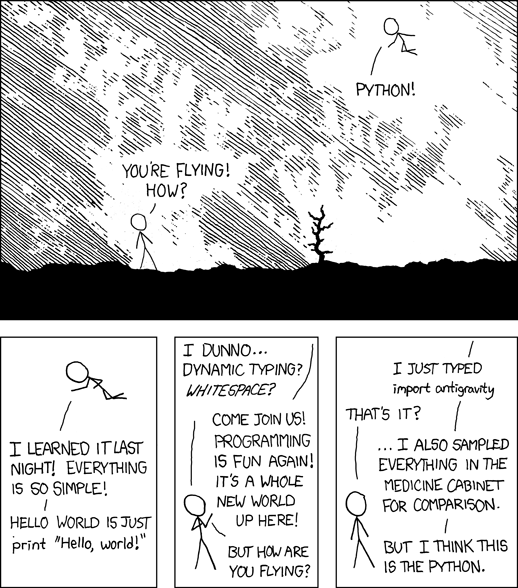
\includegraphics[width=0.5\linewidth]{figures/python.png}
\caption{$\tt{Python}$ has many modules for download on the web\ldots{}}
\label{fig:fancy_module}
\end{figure}

In Chapters~\ref{sec:datetime} and~\ref{sec:datamanip} we take a closer look at three modules which are particularly 
useful in financial analysis.

In order to load a module in a \(\tt{python}\) program you have to use the \(\tt{import}\) keyword. 
To inspect a module (to understand which are its functionalities) it can be used either 
\(\tt{help}\) and \(\tt{dir}\) keywords: the first writes a help message which usually describes 
the functionalities of the module, the latter systematically lists all the available functions of a module.
\textbf{In order to access a function of a module you have to use the dot (\texttt{.}) operator: 
\texttt{module-name.function-name}.}

The \texttt{math} module implements the most common mathematical functions, let's see an example. 

\begin{codebox}            
\begin{Verbatim}[commandchars=\\\{\}]
\PY{k+kn}{import} \PY{n+nn}{math}
\PY{n+nb}{dir}\PY{p}{(}\PY{n}{math}\PY{p}{)}

 ['\_\_doc\_\_',
  '\_\_loader\_\_',
  '\_\_name\_\_',
  '\_\_package\_\_',
  '\_\_spec\_\_',
  'acos',
  'acosh',
  'asin',
  'asinh',
  'atan',
  'atan2',
  'atanh',
  'ceil',
  'copysign',
  'cos',
  'cosh',
...
\end{Verbatim}
\end{codebox}

\begin{codebox}            
\begin{Verbatim}[commandchars=\\\{\}]
\PY{n+nb}{help}\PY{p}{(}\PY{n}{math}\PY{p}{)}

Help on module math:

NAME
    math

MODULE REFERENCE
    https://docs.python.org/3.6/library/math

    The following documentation is automatically generated from the Python
    source files.  It may be incomplete, incorrect or include features that
    are considered implementation detail and may vary between Python
    implementations.  When in doubt, consult the module reference at the
    location listed above.

DESCRIPTION
    This module is always available.  It provides access to the
    mathematical functions defined by the C standard.

FUNCTIONS
    acos({\ldots})
        acos(x)

        Return the arc cosine (measured in radians) of x.
...
\end{Verbatim}
\end{codebox}

\begin{codebox}            
\begin{Verbatim}[commandchars=\\\{\}]
\PY{n}{math}\PY{o}{.}\PY{n}{log}\PY{p}{(}\PY{l+m+mi}{3}\PY{p}{)}

1.0986122886681098
\end{Verbatim}
\end{codebox}

\begin{codebox}            
\begin{Verbatim}[commandchars=\\\{\}]
\PY{n}{math}\PY{o}{.}\PY{n}{exp}\PY{p}{(}\PY{l+m+mi}{3}\PY{p}{)}

20.085536923187668
\end{Verbatim}
\end{codebox}

\begin{codebox}            
\begin{Verbatim}[commandchars=\\\{\}]
\PY{n+nb}{print} \PY{p}{(}\PY{n+nb}{type}\PY{p}{(}\PY{n}{math}\PY{o}{.}\PY{n}{log}\PY{p}{)}\PY{p}{)} \PY{c+c1}{\PYZsh{} yet another type: builtin function}
\PY{n+nb}{print} \PY{p}{(}\PY{n+nb}{type}\PY{p}{(}\PY{n}{math}\PY{o}{.}\PY{n}{log}\PY{p}{(}\PY{l+m+mi}{3}\PY{p}{)}\PY{p}{)}\PY{p}{)}

<class 'builtin\_function\_or\_method'>
<class 'float'>
\end{Verbatim}
\end{codebox}

If you want to avoid to type \texttt{math.} every time you compute a logarithm or an exponential, 
it is possible to import only the needed functions from the module using the following syntax:

\begin{codebox}            
\begin{Verbatim}[commandchars=\\\{\}]
\PY{k+kn}{from} \PY{n+nn}{math} \PY{k}{import} \PY{n}{log}\PY{p}{,} \PY{n}{exp}
\PY{n+nb}{print} \PY{p}{(}\PY{n}{log}\PY{p}{(}\PY{l+m+mi}{3}\PY{p}{)}\PY{p}{)}
\PY{n+nb}{print} \PY{p}{(}\PY{n}{exp}\PY{p}{(}\PY{l+m+mi}{3}\PY{p}{)}\PY{p}{)}

1.0986122886681098
20.085536923187668
\end{Verbatim}
\end{codebox}

As an example let's compute the interest rate \(r\) that produces a return \(R\) of 
\euro 11000 when investing \euro 10000 for 2 years:

\[R = N\mathrm{e}^{r\tau} \implies r = \frac{1}{\tau} \mathrm{log}(\frac{R}{N})\]

\begin{codebox}            
\begin{Verbatim}[commandchars=\\\{\}]
\PY{n}{rate} \PY{o}{=} \PY{p}{(}\PY{l+m+mi}{1}\PY{o}{/}\PY{l+m+mi}{2}\PY{p}{)}\PY{o}{*}\PY{n}{log}\PY{p}{(}\PY{l+m+mf}{11000}\PY{o}{/}\PY{l+m+mi}{10000}\PY{p}{)}
\PY{n+nb}{print} \PY{p}{(}\PY{n}{rate}\PY{p}{)}

0.04765508990216247
\end{Verbatim}
\end{codebox}

\section{Indented Blocks and Conditionals}
\label{indented-blocks-and-the-ttifelse-statement}

Unlike other languages which uses parenthesis to isolate blocks of code $\tt{python}$ 
uses \emph{indentation}. A first example of this peculiarity is given by conditional statements 
(i.e. $\tt{if/elif/else}$). Such commands allow to dynamically run different blocks of code 
based on conditions. For example in the following we print different statements according to 
the value of \texttt{x}, note that the block of code to be run according each condition 
is shifted (i.e. indented) with respect to the rest of the code:

\begin{codebox}            
\begin{Verbatim}[commandchars=\\\{\}]
\PY{n+nb}{print} \PY{p}{(}\PY{n}{x}\PY{p}{)}
\PY{k}{if} \PY{n}{x} \PY{o}{==} \PY{l+m+mi}{1}\PY{p}{:} 
    \PY{n+nb}{print} \PY{p}{(}\PY{l+s+s2}{\PYZdq{}}\PY{l+s+s2}{This will not be printed}\PY{l+s+s2}{\PYZdq{}}\PY{p}{)} 
    \PY{c+c1}{\PYZsh{} the block of code that is run if the first condition is met is indented}
\PY{k}{elif} \PY{n}{x} \PY{o}{==} \PY{l+m+mi}{15}\PY{p}{:}
    \PY{n+nb}{print} \PY{p}{(}\PY{l+s+s2}{\PYZdq{}}\PY{l+s+s2}{This will not be printed either}\PY{l+s+s2}{\PYZdq{}}\PY{p}{)}
    \PY{c+c1}{\PYZsh{} again the block of code that is run here is indented}
    \PY{c+c1}{\PYZsh{} to be \PYZdq{}isolated\PYZdq{} by the rest }
\PY{k}{else}\PY{p}{:}
    \PY{n+nb}{print} \PY{p}{(}\PY{l+s+s2}{\PYZdq{}}\PY{l+s+s2}{This *will* be printed}\PY{l+s+s2}{\PYZdq{}}\PY{p}{)}

16
This *will* be printed
\end{Verbatim}
\end{codebox}

If by mistake the indentation of a block is missing an error is raised:
\begin{codebox}            
\begin{Verbatim}[commandchars=\\\{\}]
\PY{k}{if} \PY{n}{x} \PY{o}{==} \PY{l+m+mi}{1}\PY{p}{:} 
\PY{n+nb}{print} \PY{p}{(}\PY{l+s+s2}{\PYZdq{}}\PY{l+s+s2}{This will not be printed}\PY{l+s+s2}{\PYZdq{}}\PY{p}{)}
\PY{k}{elif} \PY{n}{x} \PY{o}{==} \PY{l+m+mi}{15}\PY{p}{:}
    \PY{n+nb}{print} \PY{p}{(}\PY{l+s+s2}{\PYZdq{}}\PY{l+s+s2}{This will not be printed either}\PY{l+s+s2}{\PYZdq{}}\PY{p}{)}
\PY{k}{else}\PY{p}{:}
    \PY{n+nb}{print} \PY{p}{(}\PY{l+s+s2}{\PYZdq{}}\PY{l+s+s2}{This *will* be printed}\PY{l+s+s2}{\PYZdq{}}\PY{p}{)}

File "<ipython-input-38-4535a45a6419>", line 3
  print ("This will not be printed")
    \^{}
IndentationError: expected an indented block
\end{Verbatim}
\end{codebox}

Below another example:
\begin{codebox}            
\begin{Verbatim}[commandchars=\\\{\}]
\PY{k}{if} \PY{n}{x} \PY{o}{!=} \PY{l+m+mi}{1}\PY{p}{:}
   \PY{n+nb}{print} \PY{p}{(}\PY{l+s+s2}{\PYZdq{}}\PY{l+s+s2}{x does not equal to 1}\PY{l+s+s2}{\PYZdq{}}\PY{p}{)}

x does not equal to 1
\end{Verbatim}
\end{codebox}

Just for comparison this is the same code written in $\tt{C++}$:

\begin{Shaded}
\begin{Highlighting}[]
\ControlFlowTok{if}\NormalTok{ (x == }\DecValTok{1}\NormalTok{) \{}
\NormalTok{ print (}\StringTok{"This will not be printed"}\NormalTok{);}
\NormalTok{\}}
\ControlFlowTok{else} \ControlFlowTok{if}\NormalTok{ (x == }\DecValTok{15}\NormalTok{) \{}
\NormalTok{  print (}\StringTok{"This will not be printed either"}\NormalTok{);}
\NormalTok{\}}
\ControlFlowTok{else}\NormalTok{ \{}
\NormalTok{print (}\StringTok{"This *will* be printed"}\NormalTok{);}
\NormalTok{\}}
\end{Highlighting}
\end{Shaded}
Notice how indentation doesn't matter at all here since the blocks are enclosed and 
defined by the brackets.

\section{Loops}\label{loops}

Another very important feature of a language is the ability to repeatedly run the same 
block of code many times. This is called looping and in \(\tt{python}\) can be done
 with $\tt{for}$ or $\tt{while}$ keywords.

\subsection{\texttt{for}}\label{for}

In a \texttt{for} loop we specify the set (or interval) over which we want to loop and a 
variable will assume all the values in that set (or interval). For example let's assume we 
want to print all the numbers between 25 and 30 (excluded) 

\begin{codebox}            
\begin{Verbatim}[commandchars=\\\{\}]
\PY{k}{for} \PY{n}{i} \PY{o+ow}{in} \PY{n+nb}{range}\PY{p}{(}\PY{l+m+mi}{25}\PY{p}{,} \PY{l+m+mi}{30}\PY{p}{)}\PY{p}{:}
     \PY{n+nb}{print} \PY{p}{(}\PY{n}{i}\PY{p}{)}

25
26
27
28
29
\end{Verbatim}
\end{codebox}
\noindent
where the keyword $\tt{range}$ returns the list of integers between the specified limits, 
if the first limit is not specified 0 is assumed.
At each cycle of the loop the variable $\tt{i}$ takes one of the values between
25 and 29. 

With $\tt{range}$ it is also possible to specify the step, so that the loop can jump every 2 units or to go in descending order:

\begin{codebox}            
\begin{Verbatim}[commandchars=\\\{\}]
\PY{k}{for} \PY{n}{i} \PY{o+ow}{in} \PY{n+nb}{range} \PY{p}{(}\PY{l+m+mi}{30}\PY{p}{,} \PY{l+m+mi}{25}\PY{p}{,} \PY{o}{\PYZhy{}}\PY{l+m+mi}{1}\PY{p}{)}\PY{p}{:}
    \PY{n+nb}{print} \PY{p}{(}\PY{n}{i}\PY{p}{)}

30
29
28
27
26
\end{Verbatim}
\end{codebox}

If it is needed to skip values in the loop the $\tt{continue}$ keyword can be used; 
in the code below 5 is actually not printed since it has been skipped by the condition executing 
$\tt{continue}$:

\begin{codebox}            
\begin{Verbatim}[commandchars=\\\{\}]
\PY{k}{for} \PY{n}{i} \PY{o+ow}{in} \PY{n+nb}{range}\PY{p}{(}\PY{l+m+mi}{10}\PY{p}{)}\PY{p}{:}
    \PY{k}{if} \PY{n}{i} \PY{o}{==} \PY{l+m+mi}{5}\PY{p}{:}
        \PY{k}{continue} 
    \PY{n+nb}{print} \PY{p}{(}\PY{n}{i}\PY{p}{)}

0
1
2
3
4
6
7
8
9
\end{Verbatim}
\end{codebox}

Instead of using $\tt{range}$ it is possible to specify directly the set of looping values:

\begin{codebox}            
\begin{Verbatim}[commandchars=\\\{\}]
\PY{k}{for} \PY{n}{i} \PY{o+ow}{in} \PY{p}{(}\PY{l+m+mi}{4}\PY{p}{,} \PY{l+m+mi}{6}\PY{p}{,} \PY{l+m+mi}{10}\PY{p}{,} \PY{l+m+mi}{20}\PY{p}{)}\PY{p}{:} \PY{c+c1}{\PYZsh{} here we loop directly on a list of numbers}
   \PY{n+nb}{print} \PY{p}{(}\PY{n}{i}\PY{p}{)}

4
6
10
20
\end{Verbatim}
\end{codebox}

Finally looping on a string actually means to loop on each single character:
 
\begin{codebox}            
\begin{Verbatim}[commandchars=\\\{\}]
\PY{n}{phrase} \PY{o}{=} \PY{l+s+s1}{\PYZsq{}}\PY{l+s+s1}{how to loop over a string}\PY{l+s+s1}{\PYZsq{}}
\PY{k}{for} \PY{n}{c} \PY{o+ow}{in} \PY{n}{phrase}\PY{p}{:}
   \PY{n+nb}{print} \PY{p}{(}\PY{n}{c}\PY{p}{)}

h
o
w
 
t
o
 
l
o
o
p
 
o
v
e
r
 
a
 
s
t
r
i
n
g
\end{Verbatim}
\end{codebox}

\subsection{\texttt{while}}\label{while}

The \texttt{while} statement repeats the same block of code until a condition is met.
For example in the following code, the block is run until \texttt{x} squared is less than 50.
At the beginning \texttt{x=1} and at each iteration we increment it by 1 "while" the condition 
is \texttt{True} (it should stop when $\tt{x}\gt 7$ because it is the last squared lower than 50):

\begin{codebox}            
\begin{Verbatim}[commandchars=\\\{\}]
\PY{n}{x} \PY{o}{=} \PY{l+m+mi}{1}
\PY{k}{while} \PY{n}{x} \PY{o}{*}\PY{o}{*} \PY{l+m+mi}{2} \PY{o}{\PYZlt{}} \PY{l+m+mi}{50}\PY{p}{:}
   \PY{n+nb}{print} \PY{p}{(}\PY{n}{x}\PY{p}{)}
   \PY{n}{x} \PY{o}{+}\PY{o}{=} \PY{l+m+mi}{1}

1
2
3
4
5
6
7
\end{Verbatim}
\end{codebox}

It is possible to exit prematurely from a \texttt{while} loop using the $\tt{break}$ keyword. 
In this case the while-condition is simply \texttt{True} so the code would run forever 
unless we set an exit strategy.

\begin{codebox}            
\begin{Verbatim}[commandchars=\\\{\}]
\PY{n}{x} \PY{o}{=} \PY{l+m+mi}{1}
\PY{k}{while} \PY{k+kc}{True}\PY{p}{:}
  \PY{k}{if} \PY{p}{(}\PY{n}{x} \PY{o}{*}\PY{o}{*} \PY{l+m+mi}{2} \PY{o}{\PYZgt{}} \PY{l+m+mi}{50}\PY{p}{)}\PY{p}{:} 
      \PY{k}{break}
  \PY{n+nb}{print} \PY{p}{(}\PY{n}{x}\PY{p}{)}
  \PY{n}{x} \PY{o}{+}\PY{o}{=} \PY{l+m+mi}{1} 

1
2
3
4
5
6
7
\end{Verbatim}
\end{codebox}

\section{Errors and Exceptions}
In the previous Sections we have already found a couple of examples with errors.
Here we are going to look deeply what they are and how can be managed.
There are (at least) two distinguishable kinds of errors:  \emph{syntax errors} and \emph{exceptions}.

\subsection{Syntax Errors}
Syntax errors are perhaps the most common kind of complaint you get while you are still learning \texttt{python}.

\begin{codebox}
\begin{Verbatim}[commandchars=\\\{\}]
\PY{k}{while} \PY{k+kc}{True} 
    \PY{n+nb}{print}\PY{p}{(}\PY{l+s+s1}{\PYZsq{}}\PY{l+s+s1}{Hello world}\PY{l+s+s1}{\PYZsq{}}\PY{p}{)}
	
File "<ipython-input-1-2b688bc740d7>", line 1
while True print('Hello world')
	       ^
SyntaxError: invalid syntax
\end{Verbatim}
\end{codebox}

The parser repeats the offending line and displays a little "arrow" 
pointing at the earliest point in the line where the error was detected. 
The error is caused by the token preceding the arrow: in the example, 
the error is detected at the function \texttt{print()}, 
since a colon (\texttt{:}) is missing before it. 
File name and line number are printed so you know where to look in case the input came from a script.

\subsection{Exceptions}
Even if a statement or expression is syntactically correct, it may cause 
an error when an attempt is made to execute it. 
Errors detected during execution are called exceptions and are not unconditionally fatal.
Most exceptions are not handled by programs and result in error 
messages as shown here:

\begin{codebox}
\begin{Verbatim}[commandchars=\\\{\}]
\PY{l+m+mi}{10} \PY{o}{*} \PY{p}{(}\PY{l+m+mi}{1}\PY{o}{/}\PY{l+m+mi}{0}\PY{p}{)}

---------------------------------------------------------------------------
ZeroDivisionError                         Traceback (most recent call last)

<ipython-input-2-f858149a2d27> in <module>
----> 1 10 * (1/0)

ZeroDivisionError: division by zero

\PY{l+m+mi}{4} \PY{o}{+} \PY{n}{spam}\PY{o}{*}\PY{l+m+mi}{3}

---------------------------------------------------------------------------
NameError                                 Traceback (most recent call last)

<ipython-input-3-c98bb92cdcac> in <module>
----> 1 4 + spam*3

NameError: name 'spam' is not defined

\PY{l+s+s1}{\PYZsq{}}\PY{l+s+s1}{2}\PY{l+s+s1}{\PYZsq{}} \PY{o}{+} \PY{l+m+mi}{2}

---------------------------------------------------------------------------
TypeError                                 Traceback (most recent call last)

<ipython-input-4-d2b23a1db757> in <module>
----> 1 '2' + 2

TypeError: must be str, not int
\end{Verbatim}
\end{codebox}

The last line of the error message indicates what happened. 
Exceptions come in different types, and the type is printed as part 
of the message: the types in the example are 
\texttt{ZeroDivisionError}, \texttt{NameError} and \texttt{TypeError}.
The string printed as the exception type is the name of the exception that occurred. 
The rest of the line provides detail based on the type of exception and what caused it.

The preceding part of the error message shows the context where the 
exception occurred, in the form of a stack traceback listing source lines.

\subsection{Handling Exceptions}
It is possible to write programs that handle selected exceptions. 
Look at the following example, which asks the user for input until 
a valid integer has been entered, but allows the user to interrupt 
the program (e.g. using Control-C); note that a user-generated 
interruption is signaled by raising the \texttt{KeyboardInterrupt} exception.

\begin{codebox}
\begin{Verbatim}[commandchars=\\\{\}]
\PY{k}{while} \PY{k+kc}{True}\PY{p}{:}
    \PY{k}{try}\PY{p}{:}
        \PY{n}{x} \PY{o}{=} \PY{n+nb}{int}\PY{p}{(}\PY{n+nb}{input}\PY{p}{(}\PY{l+s+s2}{\PYZdq{}}\PY{l+s+s2}{Please enter a number: }\PY{l+s+s2}{\PYZdq{}}\PY{p}{)}\PY{p}{)}
	    \PY{k}{break}
    \PY{k}{except} \PY{n+ne}{ValueError}\PY{p}{:}
        \PY{n+nb}{print}\PY{p}{(}\PY{l+s+s2}{\PYZdq{}}\PY{l+s+s2}{Oops!  That was no valid number.  Try again...}\PY{l+s+s2}{\PYZdq{}}\PY{p}{)}
	
Please enter a number: pippo
Oops!  That was no valid number.  Try again...

Please enter a number:
---------------------------------------------------------------------------

KeyboardInterrupt                         Traceback (most recent call last)
...

\end{Verbatim}
\end{codebox}

The \texttt{try} statement works as follows: first, the try clause is executed.
If no exception occurs, the except clause is skipped and 
execution of the \texttt{try} statement is finished.

If an exception occurs during execution of the try clause, 
the rest of the clause is skipped. Then if its type matches the 
exception named after the \texttt{except} keyword, the corresponding except clause 
is executed, and then execution continues after the \texttt{try} statement.

If an exception occurs which does not match the exception named in the 
except clause, it is passed on to outer \texttt{try} statements; 
if no handler is found, it is an un-handled exception and execution stops 
with a message as shown above.

A \texttt{try} statement may have more than one except clause, 
to specify handlers for different exceptions. At most one handler will be
executed. Handlers only handle exceptions that occur in the corresponding 
try clause, not in other handlers of the same \texttt{try} statement.

\begin{codebox}
	\begin{Verbatim}[commandchars=\\\{\}]
	\PY{k}{except} \PY{p}{(}\PY{n+ne}{RuntimeError}\PY{p}{,} \PY{n+ne}{TypeError}\PY{p}{,} \PY{n+ne}{NameError}\PY{p}{)}\PY{p}{:}
	\PY{k}{pass}
	\end{Verbatim}
\end{codebox}

The last except clause may omit the exception name(s), to serve as a wildcard.
Use this with extreme caution, since it is easy to mask a real programming 
error in this way! 

\begin{codebox}
	\begin{Verbatim}[commandchars=\\\{\}]
\PY{k+kn}{import} \PY{n+nn}{sys}
	
\PY{k}{try}\PY{p}{:}
    \PY{k}{with} \PY{n+nb}{open}\PY{p}{(}\PY{l+s+s1}{\PYZsq{}}\PY{l+s+s1}{myfile.txt}\PY{l+s+s1}{\PYZsq{}}\PY{p}{)} \PY{k}{as} \PY{n}{f}\PY{p}{:}
        \PY{n}{s} \PY{o}{=} \PY{n}{f}\PY{o}{.}\PY{n}{readline}\PY{p}{(}\PY{p}{)}
        \PY{n}{i} \PY{o}{=} \PY{n+nb}{int}\PY{p}{(}\PY{n}{s}\PY{o}{.}\PY{n}{strip}\PY{p}{(}\PY{p}{)}\PY{p}{)}
\PY{k}{except} \PY{n+ne}{OSError} \PY{k}{as} \PY{n}{err}\PY{p}{:}
    \PY{n+nb}{print}\PY{p}{(}\PY{l+s+s2}{\PYZdq{}}\PY{l+s+s2}{OS error: }\PY{l+s+si}{\PYZob{}0\PYZcb{}}\PY{l+s+s2}{\PYZdq{}}\PY{o}{.}\PY{n}{format}\PY{p}{(}\PY{n}{err}\PY{p}{)}\PY{p}{)}
\PY{k}{except} \PY{n+ne}{ValueError}\PY{p}{:}
    \PY{n+nb}{print}\PY{p}{(}\PY{l+s+s2}{\PYZdq{}}\PY{l+s+s2}{Could not convert data to an integer.}\PY{l+s+s2}{\PYZdq{}}\PY{p}{)}
\PY{k}{except}\PY{p}{:}
    \PY{n+nb}{print}\PY{p}{(}\PY{l+s+s2}{\PYZdq{}}\PY{l+s+s2}{Unexpected error:}\PY{l+s+s2}{\PYZdq{}}\PY{p}{,} \PY{n}{sys}\PY{o}{.}\PY{n}{exc\PYZus{}info}\PY{p}{(}\PY{p}{)}\PY{p}{[}\PY{l+m+mi}{0}\PY{p}{]}\PY{p}{)}
	
OS error: [Errno 2] No such file or directory: 'myfile.txt'
\end{Verbatim}
\end{codebox}

\section{Exercises}
\begin{question}
What is the built-in function that \(\tt{python}\) uses to iterate over a number sequence ? Write an example that uses it.
\end{question}

\cprotEnv \begin{solution}
The built-in function used to iterate over a sequence of numbers is \(\tt{range}\). It returns a sequence of numbers taking three parameters that represents respectively the lower boundary of the sequence, the upper boundary of the sequence and the step. Note that the upper boundary is excluded from the sequence.

\begin{ipython}
for i in range(10, 20, 2):
    print (i)
\end{ipython}
\begin{ioutput}
10
12
14
16
18
\end{ioutput}
If just one parameter is passed the default lower boundary is 0 and the step is 1. 
\begin{ipython}
for i in range(5):
    print (i)
\end{ipython}
\begin{ioutput}    
0
1
2
3
4
\end{ioutput}
\end{solution}

\begin{question}
What is a string in \(\tt{python}\) ? Declare one string variable and try to manipulate it (concatenate, make uppercase, capitalize, replace characters, split...).
\end{question}

\cprotEnv \begin{solution}
A string is simply a sequence of characters.

\begin{ipython}
aString = "this is a string"
  
aString = aString + ", just an example"
print(aString)
\end{ipython}
\begin{ioutput}
'this is a string, just an example'
\end{ioutput}
\begin{ipython}
print(aString.upper())
\end{ipython}
\begin{ioutput}
'THIS IS A STRING, JUST AN EXAMPLE'
\end{ioutput}
\begin{ipython}
print(aString.capitalize())
\end{ipython}
\begin{ioutput}
'This is a string, just an example'
\end{ioutput}
\begin{ipython}
print(aString.replace("just an", "for"))
\end{ipython}
\begin{ioutput}
'this is a string, for example'
\end{ioutput}
\begin{ipython}
print(aString.split(","))
\end{ipython}
\begin{ioutput}
['this is a string', ' just an example']
\end{ioutput}
\begin{ipython}
if aString.endswith("example"):
    print("This string is really an example.")
else:
    print("This string is not an example.")
\end{ipython}
\begin{ioutput}
'This string is really an example.'
\end{ioutput}
\end{solution}

\begin{question}
What does the continue do in \(\tt{python}\) ? Show an example of its usage printing all the odd numbers between 0 and 10.
\end{question}

\cprotEnv \begin{solution}
\(\tt{continue}\) is used to skip cycles in for loops. Note that \% is the module operator, it returns the reminder of a division.

\begin{ipython}
for i in range(10):
    if i%2 == 0:
        continue
    else:
        print(i)
\end{ipython}
\begin{ioutput}    
1
3
5
7
9
\end{ioutput}
\end{solution}

\begin{question}
When should you use the break in \(\tt{python}\) ? Show an example of its usage.
\end{question}

\cprotEnv \begin{solution}
\(\tt{break}\) is the command used to interrupt a while loop even if the while condition is still satisfied.

\begin{ipython}
i = 0
while i < 11:
    if (i/2) > 3:
        break
    print(i)
    i += 1 
\end{ipython}
\begin{ioutput}    
0
1
2
3
4
5
6
\end{ioutput}
\end{solution}

\begin{question}
Which \(\tt{python}\) function will you use to convert a number to a string ? Show an example.
\end{question}

\cprotEnv \begin{solution}
\(\tt{str()}\) is the correct function to use in order to cast a number to a string.

\begin{ipython}
x = 2.34
print("This {} is of type {}".format(x, type(x)))
print("This {} is of type {}".format(str(x), type(str(x))))
\end{ipython}
\begin{ioutput}    
This 2.34 is of type <class 'float'>
This 2.34 is of type <class 'str'>
\end{ioutput}
\end{solution}

\begin{question}
Import the math module and compute the logarithm of 2.09, the exponential of 1.57 and the area of a circle of radius 6 cm (circle area = $\pi \cdot r^2$).
\end{question}

\cprotEnv \begin{solution}
\begin{ipython}
import math

print ("log(2.09) = {}".format(math.log(2.09))
print ("exp(1.57) = {}".format(math.exp(1.57))
print ("area of a circle (R=6cm) is about {} cm2".format(math.pi*6*6))
\end{ipython}
\begin{ioutput}    
log(2.09) = 0.7371640659767196
exp(1.57) = 4.806648193775178
area of circle (R=6cm) is about 113.10 cm2
\end{ioutput}
\end{solution}

\cprotEnv \begin{question}
\label{ex:BS1}
Given the following variables write out the Black Scholes formula and save the value of a call in a variable named `call\_price' and the value of a put in a variable named `put\_price'.

\begin{ipython}
S_t = 800.0 # spot price of the underlying
K = 600.0 # strike price
vol = 0.25 # volatility
r = 0.01 # interest rate
ttm = 0.5 # time to maturity, in years
\end{ipython}
\textbf{Hint:} remember that there are many modules available in \texttt{python} that let you save a lot of time. In this case we need the cumulative distribution function of the standard normal distribution which can be found in \texttt{scipy.stats} module, the name of the function is \texttt{norm}.
\end{question}

\cprotEnv \begin{solution}
The BS equation for the price of a call is:

\[ C(S, t) = S_tN(d_1)-Ke^{-r(T-t)}N(d_2) \]

where
\begin{itemize}
\item \(S_t\) is the spot price of the underlying
\item \(K\) is the strike price
\item \(r\) is the risk-free interest rate (expressed in terms of continuous compounding)
\item \(N(\cdot)\) is the cumulative distribution function of the standard normal distribution
\item \(T - t\) is the time to maturity
\item \(\sigma\) is the volatility of the underlying
\end{itemize}

\[\begin{split}
d_1 & = \cfrac{\mathrm{ln}(\cfrac{S_t}{K}) + (r + \cfrac{1}{2}\sigma^{2})(T-t)}{\sigma\sqrt{T-t}}\\ \\
d_2 & = d_1 - \sigma\sqrt{T-t}\\
\end{split}\]

\begin{ipython}
from math import log, exp, sqrt
# You'll need the Gaussian cumulative distribution function 
from scipy.stats import norm

S_t = 800.0 
ttm = 0.5
K = 600.0 
vol = 0.25 
r = 0.01

d1_num = (log(S_t/K)+(r+0.5*pow(vol, 2))*ttm) 
d1_den = vol*sqrt(ttm)
d1 = d1_num /d1_den
d2 = d1 - d1_den

call_price = S_t * norm.cdf(d1) - K * exp(-r*ttm)*norm.cdf(d2)
put_price = - S_t * norm.cdf(-d1) + K * exp(-r*ttm)*norm.cdf(-d2)
print ("{:.3f} {:.3f}".format(call_price, put_price)) 
\end{ipython}
\begin{ioutput}    
205.472 2.480
\end{ioutput}
\end{solution}


\begin{thebibliography}{9}
%\bibitem{survey2019} StackOverflow \emph{The TEXbook}, Addison-Wesley, Reading,Massachusetts, second edition, 1984,
\bibitem{survey2019} \href{https://insights.stackoverflow.com/survey/2019}{\emph{Stack Overflow 2019 survey}}, Stack Overflow, 2019 [Online]
\bibitem{python_versions} \href{https://www.python.org/downloads/}{\emph{Python Distribution Versions}}, \texttt{python.org} [Online]
\bibitem{learn_python} \href{https://www.learnpython.org/it/}{\emph{Learning Python}}, \texttt{learnpython.org} [Online]
\bibitem{freecamp} \href{https://www.youtube.com/watch?v=8DvywoWv6fI}{\emph{Python Basics Tutorial}}, \texttt{freeCodeCamp.org} [Online]
\bibitem{modules} \href{https://docs.python.org/3/py-modindex.html}{\emph{Complete list of Python 3 modules}} [Online]
\end{thebibliography}
